\chapter{集合和常用逻辑用语}

数学在从算术演化到现代的数学的过程中,逻辑起到了关键性作用。逻辑的发展使得数学从具体的对数和形的讨论上升到对抽象思维的分析和判断。

本章讨论现代数学思维的两大基础——集合和逻辑用语。集合是对考察对象的框定,即我们总是对一类限定的事物进行思考。逻辑用语表示了我们总是按照一定的方法进行思考。

本章要点:
\begin{itemize}
    \item 集合及其运算法则。
    \item 充分条件和必要条件。
    \item 全称量词和存在量词。
\end{itemize}

\newpage
\section{集合的概念}

本节要点:
\begin{itemize}
    \item 掌握集合的概念;
    \item 熟练掌握集合的描述法。
\end{itemize}

~

集合的概念并没有什么难度,重在理解元素。元素可以是数、点、或者任何可以准确描述的事物,但必须满足:
\begin{itemize}
    \item {\bf 确定性}:元素$a$要么在集合$A$中,要么不在$A$中,逻辑上必须清晰;
    \item {\bf 唯一性}:集合$A$中不能存在两个一模一样的元素,用数学语言表达就是$\forall a,b\in A,a\ne b$;
    \item {\bf 无序性}:集合$A$中的元素$a$和$b$,我们只讨论其存在,不关心它们的顺序。
\end{itemize}

对于集合的表示方法,教材写地有些凌乱。掌握一点,数学中,我们用花括号描述集合,如:
\[
A=\left\{ \text{这是一个集合} \right\}
\]
花括号中的描述方法没有特别的格式规范,只要求明确清晰即可。一般地,我们用竖线分割,前半部用小写字母表示元素,后半部用表达式确定元素的范围或关系等限定,如果有多个限定,则用逗号分隔,如下:
\begin{align*}
&A=\left\{ x \middle| x>3 \right\} \\
&B=\left\{ \left( x,y \right) \middle| x^2+y^2>1 \right\} \\
&C=\left\{ x \middle| x\in \mathbb{R} ,x^2=-1 \right\}
\end{align*}
集合$A$表示了数轴上的一个段,其元素是单个数$x$;集合$B$表示了平面上的一个圆,其元素是平面上的点,用一个有序数对$\left( x,y \right) $表示;集合$C$描述了一个空集,和$C=\oslash $是一样的,这说明集合的描述并不唯一。

\begin{tcolorbox}
不必刻意理解教材中的列举法、描述法等方法,后面到了函数阶段,定义域、值域都是采用这种描述方法,所以只需理解并熟练掌握上述描述方法即可。
\end{tcolorbox}

\begin{tcolorbox}
广义来讲,集合和元素的概念非常宽泛,没有限定必须是数字。如我们可以将高一(2)班作为一个集合,那么班级里的同学可以视作元素。我们也可以将所有多项式组成一个集合。我们更可以将马达加斯加的雄性企鹅组成一个集合。
\end{tcolorbox}






\newpage
\section{集合间的基本关系}

本节要点:
\begin{itemize}
    \item 熟练掌握集合的各种关系。
\end{itemize}

~

集合的关系概念并没有什么难度。重点区分$a$和$\left\{ a \right\} $,前者是一个元素,后者是一个集合。

~

\begin{example}[综合运用4,难度:$\star $]
在平面直角坐标系中$C=\left\{ \left( x,y \right) \middle| y=x \right\} $表示直线$y=x$,从这个角度看,集合
\[
D=\left\{ \left( x,y \right) \middle| \left\{ \begin{array}{c}
	2x-y=1\\
	x+4y=5\\
\end{array} \right. \right\}
\]
表示什么?$C,D$间有什么关系?
\end{example}

解:

首先看$C$的表示方法$C=\left\{ \left( x,y \right) \middle| y=x \right\} $,各部分分析如下:
\begin{itemize}
    \item $C$:大写字母表示集合;
    \item $\left( x,y \right) $:一个有序实数对表示集合的元素是平面的点;
    \item $y=x$:一个等式表示$x,y$需满足的约束条件。
\end{itemize}
同理分析$D$的表示方法:
\begin{itemize}
    \item $D$:大写字母表示另一个集合;
    \item $\left( x,y \right) $:一个有序实数表示集合的元素依然是平面的点;
    \item $\left\{ \begin{array}{c}
        2x-y=1\\
        x+4y=5\\
    \end{array} \right. $:联立的两个等式表示$x,y$需要“同时”满足的两个约束条件。
\end{itemize}
不难发现,每个约束代表一条直线,若要“同时”满足两个约束条件,几何上表示两条直线的交点。
解方程组易得$x=y=1$,可见$C\supset D$。
$C,D$表示的几何图形如下:

\begin{figure}[h]
\centering
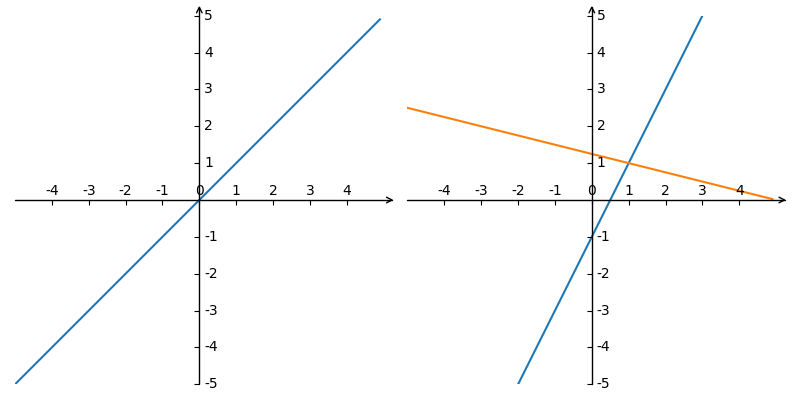
\includegraphics[height=4cm]{1.2-1.png}
\end{figure}

\begin{tcolorbox}
本题考察集合的概念和集合的描述方法。
\end{tcolorbox}






\newpage
\section{集合的基本运算}

本节要点:
\begin{itemize}
    \item 熟练掌握集合的运算法则。
\end{itemize}

~

集合的运算并没有什么难度。教材介绍了3中运算,交并补,我们可以做如下精确的定义。

\begin{definition}[集合的运算]
设三个集合$A,B,C$,若$A$中的任一元素同时属于$C$,且$B$中的任一元素也同时属于$C$,则称{\bf $C$为$A,B$的并集},记作$A\cup B$,即:
\[
A\cup B:=\left\{ a \middle| a\in A\text{或}a\in B \right\}
\]
若$C$中的任一元素同时属于$A$和$B$,则称{\bf $C$为$A,B$的交集},记作$A\cap B$,即:
\[
A\cap B:=\left\{ a \middle| a\in A\text{且}a\in B \right\}
\]
若我们将$A$中的同时属于$B$的元素去除,得到的集合称为{\bf $A$和$B$的差},也称为{\bf $B$关于$A$的补集},记作$A\cap \bar{B}$,即:
\[
A\cap \bar{B}:=\left\{ a \middle| a\in A\text{且}a\notin B \right\}
\]
\end{definition}

\begin{figure}[h]
\centering
\begin{tikzpicture}[line join=round, scale=0.5]
% A in B
\coordinate (O) at (-5,1.6);
\draw[thick] ($(O)+(-2,-1)$)--($(O)+(2,-1)$)--($(O)+(2,1)$)--($(O)+(-2,1)$)--($(O)+(-2,-1)$);
\coordinate[label=above:{$A\subset B$}] (t) at ($($(O)+(-2,1)$)!0.5!($(O)+(2,1)$)$);
\draw[thick] ($(O)+(0,0)$) ellipse (1.5 and 0.8);
\draw[thick] ($(O)+(0,0)$) circle (0.5);
\coordinate[label=center:{$A$}] (a) at ($(O)+(0,0)$);
\coordinate[label=center:{$B$}] (b) at ($(O)+(1,0)$);
% A or B
\coordinate (O) at (0,1.6);
\draw[thick] ($(O)+(-2,-1)$)--($(O)+(2,-1)$)--($(O)+(2,1)$)--($(O)+(-2,1)$)--($(O)+(-2,-1)$);
\coordinate[label=above:{$A\cup B$}] (t) at ($($(O)+(-2,1)$)!0.5!($(O)+(2,1)$)$);
\fill[black!30!white] ($(O)+(-0.5,0)$) circle (0.8);
\fill[black!30!white] ($(O)+(0.5,0)$)  circle (0.8);
\draw[thick] ($(O)+(-0.5,0)$) circle (0.8);
\draw[thick] ($(O)+(0.5,0)$)  circle (0.8);
\coordinate[label=center:{$A$}] (a) at ($(O)+(-0.7,0)$);
\coordinate[label=center:{$B$}] (b) at ($(O)+(0.7,0)$);
% A and B
\coordinate (O) at (5,1.6);
\draw[thick] ($(O)+(-2,-1)$)--($(O)+(2,-1)$)--($(O)+(2,1)$)--($(O)+(-2,1)$)--($(O)+(-2,-1)$);
\coordinate[label=above:{$A\cap B$}] (t) at ($($(O)+(-2,1)$)!0.5!($(O)+(2,1)$)$);
\begin{scope}
\clip[draw] ($(O)+(-0.5,0)$) circle (0.8);
\fill[black!30!white] ($(O)+(0.5,0)$) circle (0.8);
\end{scope}
\draw[thick] ($(O)+(-0.5,0)$) circle (0.8);
\draw[thick] ($(O)+(0.5,0)$)  circle (0.8);
\coordinate[label=center:{$A$}] (a) at ($(O)+(-0.7,0)$);
\coordinate[label=center:{$B$}] (b) at ($(O)+(0.7,0)$);
% A - B
\coordinate (O) at (-5,-1.6);
\draw[thick] ($(O)+(-2,-1)$)--($(O)+(2,-1)$)--($(O)+(2,1)$)--($(O)+(-2,1)$)--($(O)+(-2,-1)$);
\coordinate[label=above:{$A-B=A\cap \bar{B}$}] (t) at ($($(O)+(-2,1)$)!0.5!($(O)+(2,1)$)$);
\fill[black!30!white] ($(O)+(-0.5,0)$) circle (0.8);
\draw[thick,fill=white] ($(O)+(0.5,0)$) circle (0.8);
\draw[thick] ($(O)+(-0.5,0)$) circle (0.8);
\coordinate[label=center:{$A$}] (a) at ($(O)+(-0.7,0)$);
\coordinate[label=center:{$B$}] (b) at ($(O)+(0.7,0)$);
% A and B is null
\coordinate (O) at (0,-1.6);
\draw[thick] ($(O)+(-2,-1)$)--($(O)+(2,-1)$)--($(O)+(2,1)$)--($(O)+(-2,1)$)--($(O)+(-2,-1)$);
\coordinate[label=above:{$A\cap B=\oslash $}] (t) at ($($(O)+(-2,1)$)!0.5!($(O)+(2,1)$)$);
\draw[thick] ($(O)+(-0.9,0)$) circle (0.8);
\draw[thick] ($(O)+(0.9,0)$)  circle (0.8);
\coordinate[label=center:{$A$}] (a) at ($(O)+(-0.9,0)$);
\coordinate[label=center:{$B$}] (b) at ($(O)+(0.9,0)$);
% not A
\coordinate (O) at (5,-1.6);
\fill[black!30!white] ($(O)+(-2,-1)$)--($(O)+(2,-1)$)--($(O)+(2,1)$)--($(O)+(-2,1)$)--cycle;
\draw[thick] ($(O)+(-2,-1)$)--($(O)+(2,-1)$)--($(O)+(2,1)$)--($(O)+(-2,1)$)--($(O)+(-2,-1)$);
\coordinate[label=above:{$\bar{A}$}] (t) at ($($(O)+(-2,1)$)!0.5!($(O)+(2,1)$)$);
\draw[thick,fill=white] ($(O)+(0,0)$) circle (0.8);
\coordinate[label=center:{$A$}] (a) at ($(O)+(0,0)$);
\end{tikzpicture}
\end{figure}

集合的运算除逻辑符号外,还可使用算术符号描述。

\begin{table}[h]
\centering
\begin{tabular}{ccc}
    \toprule
    运算 & 逻辑符号 & 算术符号\\
    \midrule
    并 & $A\cup B$ & $A+B$\\
    交 & $A\cap B$ & $AB$\\
    差 & $A\cap \bar{B}$ & $A-B$\\
    \bottomrule
\end{tabular}
\end{table}

\begin{tcolorbox}
集合的运算使得我们可以用一些简单集合的组合描述一个复杂集合。但要注意,这里的运算是逻辑运算,而非算术运算。
\end{tcolorbox}

集合的运算法则:
\begin{itemize}
    \item {\bf 交换律}:$AB=BA$
    \item {\bf 结合律}:$\left( A+B \right) +C=A+\left( B+C \right) ,\left( AB \right) C=A\left( BC \right) $
    \item {\bf 分配律}:$\left( A+B \right) C=\left( AC \right) +\left( AB \right) ,\left( AB \right) +C=\left( A+C \right) \left( B+C \right) $
    \item {\bf 德摩根律}:$\overline{A+B}=\bar{A}\bar{B},\overline{AB}=\bar{A}+\bar{B}$
\end{itemize}

~

其他常用运算公式:
\begin{align*}
& AB\subset A\subset A+B,\qquad AB\subset B\subset A+B \\
& AA=A \\
& A+A=A \\
& A+\bar{A}=\varOmega \\
& A-B=A\bar{B}=A-AB \\
& \left( A-B \right) +B=A+B
\end{align*}

\begin{tcolorbox}
上述运算法则和公式有些超纲,有兴趣可XML。
\end{tcolorbox}






\newpage
\section{充分条件和必要条件}

本节要点:
\begin{itemize}
    \item 了解命题的概念;
    \item 熟练掌握并深刻理解充分条件和必要条件的概念。
\end{itemize}

~

命题是一个陈述句,往往很简单,而且陈述是明确的、无歧义的,命题的结论要么为真、要么为假,只有其中一个结果,而且结果也是明确的、无歧义的。

对于充分条件和必要条件,下列四种说法等价:
\begin{itemize}
    \item 命题“若$p$,则$q$”为真命题;
    \item $p\Rightarrow q$;
    \item $p$是$q$的充分条件;
    \item $q$是$p$的必要条件。
\end{itemize}

\begin{tcolorbox}
对于命题、充分条件、必要条件,我们无需从形式逻辑方面完全掌握其概念,毕竟不是逻辑课程。我们只需了解它们是如何构建数学中的定义、定理、性质的。
\end{tcolorbox}

一般来讲,定义(definition)$D$是逻辑的起点,是一个人为的设定,不容置疑的。而判断一事物是否为$D$会比较复杂,定理(theorem)$T$给出了判断事物是否为$D$的简单方法,通常定理以充分条件的形式给出。一旦我们获得了一事物是$D$这个判断,那么该事物必然有$D$的性质(property)$P$,通常这类性质往往以必要条件的形式给出。
\[
T\rightarrow D\rightarrow P
\]

具体到解题中,已知条件通常以定理的前提给出,问题则以性质的结论要求计算或证明。所以,可以总结解题套路:
\begin{enumerate}
    \item 用定理将式子或图形框在某一定义中,如证明两个三角形相似即将两个三角形框在了相似这个定义中;
    \item 用性质得出结论,如计算另一个三角形的某个角。
\end{enumerate}
\[
\text{已知}\overset{T}{\Rightarrow}D\overset{P}{\Rightarrow}\text{结论}
\]

\begin{tcolorbox}
充要条件是整个高中乃至整个数学的思维范式!需要深刻领会。如何研究事物的运动规律?这是有一套固定的方法论的。数学上,我们不会单独讨论某个问题,而是将所有类似的问题总结提炼,形成定义、定理、性质。碰到具体问题,首先将问题转到数学空间,即归类到某个数学定义,然后用那个定义配套的定理和性质分析问题。这就是西方科学的基石,从亚里士多德开始的演绎法!
\end{tcolorbox}

\begin{tcolorbox}
演绎法是由一般到特殊的推理方法,与“归纳法”相对。最著名的演绎论恐怕莫过于:所有人都会死,苏格拉底是人,所以苏格拉底会死。演绎法中,“一般”是已知的事实,“特殊”是未知的结论。数学中,这个一般的已知的事实就是我们学习的各种数学概念、定理、公式,这个特殊就是各种题目。题目千千万万,但万变不离其宗,再抽象晦涩的题目总能化为最最基础的数学概念。事实上,高中数学也就是那么几个一个手数地过来的基础概念。
\end{tcolorbox}






\newpage
\section{全称量词和存在量词}

略。






\newpage
\section{本章小结}

形而上方面,本章介绍了数学的思维范式——演绎法,在以后的学习过程中需要不断加深认识。形而下方面,本章介绍了逻辑的基本知识。集合和逻辑用语是现代数学的语言基础。本章定义了一些数学符号,如$\cap ,\cup ,\in ,\forall ,\exists $,这些符号使得数学语言脱离了自然语言,去除了自然语言的模糊性,让数学更加清晰精准。随着学习的深入,我们会定义更多的数学符号,记住,数学符号就是为了精确、准确、无歧义地表述。

我们再用数学判断命题或计算某个值时,往往使用“定理—定义—性质”这个步骤。如计算下面$\bigtriangleup ABC$的角$\alpha $,我们可以按如下步骤:
\begin{enumerate}
    \item 用定理证明$\bigtriangleup ABC$和$\bigtriangleup abc$相似;
    \item 用性质得到$\alpha =60^\circ$。
\end{enumerate}

\begin{figure}[h]
\centering
\begin{minipage}{.49\textwidth}
\centering
\begin{tikzpicture}[line join=round, scale=1]
\coordinate[label=above:{$A$}] (A) at (0.5,1);
\coordinate[label=left: {$B$}] (B) at (-1,0);
\coordinate[label=right:{$C$}] (C) at (1,0);
\draw[thick] (A)--(B)--(C)--(A);
\pic["$\alpha $",draw,angle radius=0.5cm,angle eccentricity=1.5] {angle=A--C--B};
\end{tikzpicture}
\end{minipage}
\begin{minipage}{.49\textwidth}
\centering
\begin{tikzpicture}[line join=round, scale=1.5]
\coordinate[label=above:{$a$}] (A) at (0.5,1);
\coordinate[label=left: {$b$}] (B) at (-1,0);
\coordinate[label=right:{$c$}] (C) at (1,0);
\draw[thick] (A)--(B)--(C)--(A);
\pic["$\pi /3$",draw,angle radius=0.5cm,angle eccentricity=1.8] {angle=A--C--B};
\end{tikzpicture}
\end{minipage}
\end{figure}

定义是逻辑起点,也是我们围绕的中心,是我们学习数学时的重中之重。定理是用来快速判断是否符合定义,让我们在逻辑上对定义有更深刻的认识。性质则是用来得到我们想要的结果。

~

\begin{example}[综合运用8,难度:$\star $]
已知
\begin{align*}
&A=\left\{ \left( x,y \right) \middle| 2x-y=0 \right\} \\
&B=\left\{ \left( x,y \right) \middle| 3x+y=0 \right\} \\
&C=\left\{ \left( x,y \right) \middle| 2x-y=3 \right\}
\end{align*}
求$A\cap B,A\cap C$,并解释它们的几何意义。
\end{example}

解:

\begin{align*}
&A\cap B=\left\{ \left( x,y \right) \middle| \left\{ \begin{array}{c}
	2x-y=0\\
	3x+y=0\\
\end{array} \right. \right\} \\
&A\cap C=\left\{ \left( x,y \right) \middle| \left\{ \begin{array}{c}
	2x-y=0\\
	2x-y=3\\
\end{array} \right. \right\}
\end{align*}

$A,B,C$几何上均表示平面的直线,$A\cap B$表示点即在直线$A$上也在直线$B$上,所以是它们的交点。不难发现,$A\cap B$是有交点的,但$A\cap C$表示两条平行线,没有交点。
\begin{figure}[ht]
\centering
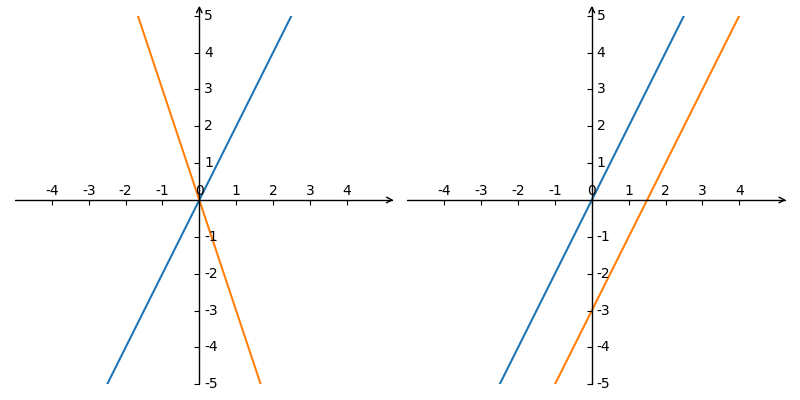
\includegraphics[height=4cm]{1.6-2.png}
\end{figure}

\begin{tcolorbox}
该题注意数形结合。
\end{tcolorbox}

~

\begin{example}[拓广探索12(2),难度:$\star \star \star $]
如图,在$\bigtriangleup ABC$中,$AD,BE,CF$分别为边$BC,AC,AB$上的高,证明$AD,BE,CF$交于点$O$。
\end{example}

解一,使用替换概念的思路:

在中学平面几何里面,我们学到过三角形有4个心:
\begin{itemize}
    \item 垂心,三角形三条高的交点;
    \item 重心,三角形三条中线的交点;
    \item 外心,三角形三条边的中垂线的交点,也是三角形外接圆的圆心;
    \item 内心,三角形三条角平分线的交点,也是三角形内切圆的圆心。
\end{itemize}
显然,在这里面最接近于三条高交点的是外心。于是,我们构建$\bigtriangleup A'B'C'$,使得$A'B'\parallel AB,A'C'\parallel AC,B'C'\parallel BC$。不难证明,$AD,BE,CF$为$\bigtriangleup A'B'C'$的中垂线,必交于一点,证毕。

\begin{figure}[h]
\centering
\begin{tikzpicture}[line join=round, scale=2.5]
\pgfmathparse{0.6/2.5}
\coordinate[label=left:       {$C'$}] (C') at (-1,0);
\coordinate[label=right:      {$B'$}] (B') at (1,0);
\coordinate[label=below:      {$A'$}] (A') at (-0.2,-1.3);
\coordinate[label=above:      {$A$}]  (A)  at ($(C')!0.5!(B')$);
\coordinate[label=below left: {$B$}]  (B)  at ($(C')!0.5!(A')$);
\coordinate[label=below right:{$C$}]  (C)  at ($(A')!0.5!(B')$);
\coordinate[label=below:      {$D$}]  (D)  at ($(B)!(A)!(C)$);
\coordinate[label=above right:{$E$}]  (E)  at ($(A)!(B)!(C)$);
\coordinate[label=above left: {$F$}]  (F)  at ($(A)!(C)!(B)$);
\draw[thick,dashed,red] (A')--(B')--(C')--(A');
\draw[thick] (A)--(B)--(C)--(A);
\draw[thick,blue,name path=l1] (A)--(D);
\draw[thick,blue,name path=l2] (B)--(E);
\draw[thick,blue] (C)--(F);
\path [name intersections={of=l1 and l2}] coordinate[label=left:$O$] (O) at (intersection-1);
\fill (O) circle (\pgfmathresult mm);
\end{tikzpicture}
\end{figure}

解二,使用替换命题的思路:

$AD$并不是垂线,只是过$O$的直线,交$BC$于$D$,证明$AD\bot BC$。

借用向量的知识,两个向量垂直等价于几何上的垂直,于是:
\begin{align*}
&\because \overrightarrow{BE}\cdot \overrightarrow{AC}=0\Rightarrow \overrightarrow{BO}\cdot \overrightarrow{AC}=0 \\
&\therefore \left( \overrightarrow{AO}-\overrightarrow{AB} \right) \cdot \overrightarrow{AC}=0 \\
&\therefore \overrightarrow{AO}\cdot \overrightarrow{AC}=\overrightarrow{AB}\cdot \overrightarrow{AC}
\end{align*}
同理:
\[
\overrightarrow{AO}\cdot \overrightarrow{AB}=\overrightarrow{AC}\cdot \overrightarrow{AB}
\]
于是:
\begin{align*}
&\because \overrightarrow{AO}\cdot \overrightarrow{AC}=\overrightarrow{AO}\cdot \overrightarrow{AB}\Rightarrow \overrightarrow{AO}\cdot \left( \overrightarrow{AC}-\overrightarrow{AB} \right) =0 \\
&\therefore \overrightarrow{AO}\cdot \overrightarrow{BC}=0
\end{align*}

\begin{tcolorbox}
解法一属于偷换概念,也是一种不错的技巧。解法二属于数形结合,用代数的方法解几何问题。
\end{tcolorbox}









